% flashcards-title: Two jumps adding seven to thirty-eight
% flashcards-desc: An open number line starts at thirty-eight, jumps two to forty, then five to forty-five.
\documentclass[dvisvgm,tikz,border=8pt]{standalone}
\usetikzlibrary{arrows.meta,patterns}

\definecolor{qraNavy}{HTML}{17324D}
\definecolor{qraBlue}{HTML}{2B6CB0}
\definecolor{qraGold}{HTML}{B7791F}
\definecolor{qraPale}{HTML}{EAF2F8}
\definecolor{qraGray}{HTML}{5C6773}

\tikzset{
  qra axis/.style={draw=qraNavy, line width=1.2pt},
  qra tick/.style={draw=qraNavy, line width=1pt},
  qra guide/.style={draw=qraGray, densely dashed, line width=0.8pt},
  qra counter/.style={circle, draw=qraNavy, fill=qraPale, line width=0.9pt, minimum size=7mm, inner sep=0pt},
  qra label/.style={font=\sffamily\bfseries, text=qraNavy},
  qra small label/.style={font=\sffamily, text=qraNavy},
}

\begin{document}
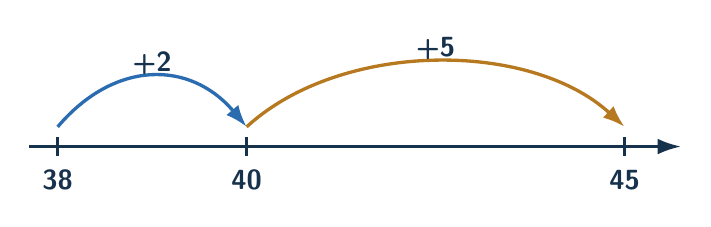
\begin{tikzpicture}[x=1.2cm,y=1cm]
  \draw[qra axis, -{Latex[length=3mm,width=2mm]}] (-0.3,0) -- (6.6,0);
  \foreach \x/\n in {0/38,2/40,6/45}{\draw[qra tick] (\x,-.12)--(\x,.12);\node[qra label,below=5pt] at (\x,0){\n};}
  \draw[qraBlue,line width=1.2pt,-{Latex[length=2.8mm,width=2mm]}] (0,.25) .. controls (0.6,1.1) and (1.4,1.1) .. (2,.25);
  \node[qra label] at (1,1.05) {+2};
  \draw[qraGold,line width=1.2pt,-{Latex[length=2.8mm,width=2mm]}] (2,.25) .. controls (3,1.35) and (5,1.35) .. (6,.25);
  \node[qra label] at (4,1.25) {+5};
\end{tikzpicture}
\end{document}
